\documentclass[conference]{IEEEtran}
\IEEEoverridecommandlockouts

\usepackage{cite}
\usepackage{amsmath,amssymb,amsfonts}
\usepackage{algorithmic}
\usepackage{graphicx}
\usepackage{textcomp}
\usepackage{tabularx}
\usepackage{subcaption}
\usepackage{xcolor}
\usepackage{listings}
\usepackage{url}
\def\BibTeX{{\rm B\kern-.05em{\sc i\kern-.025em b}\kern-.08em
    T\kern-.1667em\lower.7ex\hbox{E}\kern-.125emX}}

\title{Linguistic A-Maze-ment: Solving Textual Mazes with Pretrained Language Models}
\author{\IEEEauthorblockN{Gabriel Del Castillo\IEEEauthorrefmark{1}, Nate Webster\IEEEauthorrefmark{2}}
\IEEEauthorblockA{\textit{Department of Computer Science} \\
\textit{Colorado School of Mines}\\
Golden, CO, USA \\
\IEEEauthorrefmark{1}gdelcastillo@mines.edu,
\IEEEauthorrefmark{2}nwebster@mines.edu
}
}

\begin{document}

\maketitle

\begin{abstract}
  Large Language Models (LLMs) have shown incredible results across a wide range of natural language tasks, yet their ability to perform spatial reasoning and pathfinding remains underexplored. In this study, we evaluate the maze-solving capabilities of four pretrained LLMs—DeepSeek-V3, Gemini 2.0 Turbo, GPT-4o Mini, and LLaMA 4 Scout—using text-based maze representations generated via the \texttt{maze-dataset} library. We use a one-shot prompting strategy across 20 unique mazes, each in five distinct formats, including ASCII and various tokenized structures. Our results demonstrate significant difference in performance across models and input styles, with coordinate-based representations yielding significantly higher accuracy than cardinal-based formats. We also identify a strong inverse correlation between maze path length and solution accuracy. These findings suggest that current LLMs possess limited spatial reasoning abilities, and that input representation plays a critical role in a task's successful completion.
  
\end{abstract}

\section{Introduction}

Large Language Models (LLMs) such as GPT-4 and LlaMa 3 are able to produce remarkably accurate results when faced with various natural language processing tasks~\cite{openai}. As the scale and reach of these models have expanded, so has the focus on developing benchmarks to measure the limits and capabilities of LLMs~\cite{srivastava, liang}. However, there has been little research examining how pretrained language models handle maze solving tasks, along with identifying possible common failure patterns. The ability to solve maze-like structures has long served as a way to evaluate the cognitive and algorithmic performance of various subjects, with research ranging from rodent navigation~\cite{tolman}, to spatial understanding in infants~\cite{piaget}, to path planning for robotic systems~\cite{stentz}.

Motivated by this, as well as the prospect of integrating LLMs into physical robotic agents capable of speech, we analyze the responses of four different language models after being prompted with one of several solvable maze configurations. We evaluate the validity and optimality of their answers, and measure if parameter count, model distribution type, or maze representation have an impact on task performance.

The overarching goal of our work was to determine whether publicly available language models have sufficient spatial awareness to correctly execute a given navigational task. In turn, this serves as a foundation for deploying LLMs in contexts where they need to interact with the physical world.

\section{Related Work}
Popular LLM benchmarks, including MMLU \cite{hendrycks}, BIG-Bench \cite{srivastava}, and HELM \cite{liang} provide evaluation frameworks across several language and logic-related tasks, yet fail to test for a model's spatial reasoning or path-finding abilities. Research focused on evaluating language models in embodied settings, such as SayCan \cite{ahn} and ReAct \cite{yao}, reflects the growing interest in testing LLM's capacity for interaction beyond pure language. In addition, recent advances in automatic and customizable maze generation have made it feasible to evaluate symbolic spatial reasoning in LLMs. Specifically, the library presented in \cite{ivanitskiy} enables configurable creation and representation of maze structures, which is well-suited for benchmarking purposes.

\section{Methodology}
We evaluated four different LLMs: DeepSeek-V3~\cite{deepseek}, Gemini 2.0 Turbo~\cite{gemini}, GPT-4o Mini~\cite{gpt4omini}, and LLaMA 4 Scout~\cite{llama4scout}. These models were selected to reflect a range of parameter sizes and distribution types (e.g. open weights vs proprietary APIs), guided by the Promptmetheus LLM Index~\cite{promptmetheus}. Each was prompted through the OpenAI API~\cite{openaiapi} using the corresponding endpoints for the other providers. A summary of the models can be found in Table~\ref{tab:models}.

\begin{table}[t]
  \centering
  \caption{Language Models Evaluated in This Study}
  \begin{tabular}{|l|l|l|l|}
    \hline
    \textbf{Model} & \textbf{Provider} & \textbf{Params (Approx.)} & \textbf{Distribution} \\
    \hline
    DeepSeek-V3 & DeepSeek & 671B & Open Source \\
    Gemini 2.0 Turbo& Google & Undisclosed & Proprietary \\
    GPT-4o Mini & OpenAI & $\sim$8B (est.) & Proprietary \\
    LLaMA 4 Scout & DeepInfra & 17B & Open Weights \\
    \hline
  \end{tabular}
  \label{tab:models}
\end{table}

To accomplish our evaluation task, we generated a total of 21 unique mazes, derived from the \texttt{maze-dataset} library~\cite{ivanitskiy}, employing depth-first search generation with forks disabled. The first maze, along with its solution, were used as an in-context demonstration to allow for a one-shot prompting strategy. For each of the remaining 20 mazes, five distinct textual representations were created to test the models' ability to generalize across input formats. These included an ASCII format, and four tokenized versions using unique-token (UT) and cardinal-tuple-token (CTT) schemes. 

Prompts followed a consistent structure: a system message instructing the model to act as a maze-solving assistant, and a user message containing a solved example followed by a new maze to solve. Each model was evaluated on the same set of prompts across all representations to ensure fair comparison, which was accomplished manually.

\section{Results}
\subsection{Large Language Models Performance Summary}
As shown in Figure~\ref{fig:llm_comp}, The \texttt{deepseek-v3} model on average performs best with a total accuracy of 41\% over all input formats. It also consistently performs best on coordinate-based input formats, particularly on coordinate-based formats, with an accuracy as high as 90\% for \texttt{CTT\_Coord} inputs. However, it does perform the worst and the generally worse performing cardinal-based input formats. One interesting result is that it performs significantly better than the other models when dealing with a \texttt{ASCII} inputs with an accuracy of 20\% in comparison to the next best models' 5\%.

The \texttt{gemini-2.0-turbo} and \texttt{gpt-4o-mini} models have similar performances for each input format with total accuracies of 31\% and 36\% respectively. They are both relatively better at cardinal-based inputs over coordinate-based. The \texttt{llama-4-scout-17b-16e-instruct} model is most similar to the \texttt{deepseek-v3} model, but with the worst total accuracy of 30\%. It generally underperforms with a slightly better accuracy to the other two models on coordinate-based inputs while still being worse on cardinal-based inputs. It also has the lowest tested accuracy of 0\% when dealing with a \texttt{ASCII} inputs.

\begin{figure}[htbp]
  \centering
  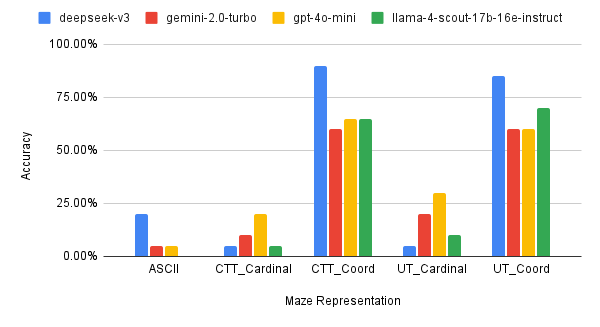
\includegraphics[width=\columnwidth]{LLM Model Comparisons for Various Maze Representations.png}
  \caption{LLM Model Comparisons for Various Maze Representations. It compares the accuracy of each of the four models for each input type of varying Coordinate Tokenizers and Adjacency List Tokenizers, as well as ASCII.}
  \label{fig:llm_comp}
\end{figure}

\subsection{Maze Input Breakdown per LLM}

According to Figure~\ref{fig:llm_maze_solution}, the worst performing mazes were Maze 3 and Maze 5. As seen in Figure~\ref{fig:worst_mazes}, the path length for these mazes is quite long, going through around half of the possible spaces. Looping back on themselves might also play a role, potentially confusing the Large Language Model to take a shortcut and skip over a wall. Both of these mazes were able to be solved by the \texttt{deepseek-v3} model in some capacity and were only solved through coordinate-based inputs, shown in Figure~\ref{fig:input_maze_solution}.

Also according to Figure~\ref{fig:llm_maze_solution}, the best performing maze was Maze 13. As seen in Figure~\ref{fig:best_maze}, the solution is extremely trivial, traveling only one space away, which is a pattern for most of the other high performing mazes. The \texttt{gpt-4o-mini} was able to solve this problem for every input format, beating out the \texttt{deepseek-v3} model, likely due to its under-performance in cardinal-based inputs. Coordinate-based inputs still outperform for this maze, shown in Figure~\ref{fig:input_maze_solution}.

\begin{figure}[htbp]
  \centering
  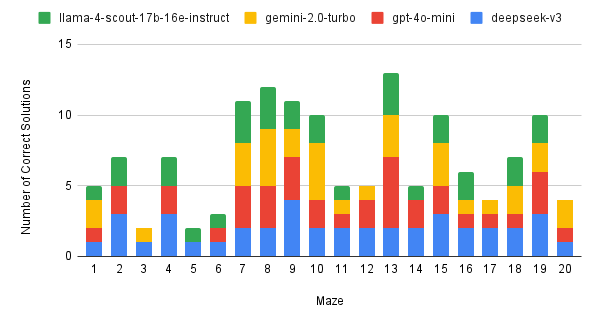
\includegraphics[width=\columnwidth]{Correct Solutions for each Maze and Large Language Model.png}
  \caption{Correct Solutions for each Maze and LLM. It highlights how each Large Language Model performed on all inputs formats of each maze}
  \label{fig:llm_maze_solution}
\end{figure}

\begin{figure}[htbp]
  \centering
  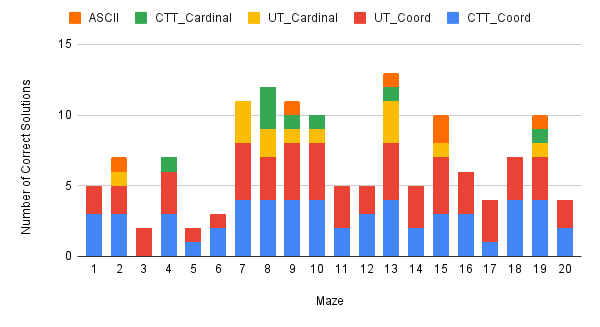
\includegraphics[width=\columnwidth]{Correct Solutions for each Maze and Input Format.png}
  \caption{Correct Solutions for each Maze and Input Format. It highlights how each input format contributed to the number of correct solutions for each Large Language Model.}
  \label{fig:input_maze_solution}
\end{figure}

\begin{figure}[htbp]
  \centering
  \begin{subfigure}[b]{0.45\columnwidth}
    \centering
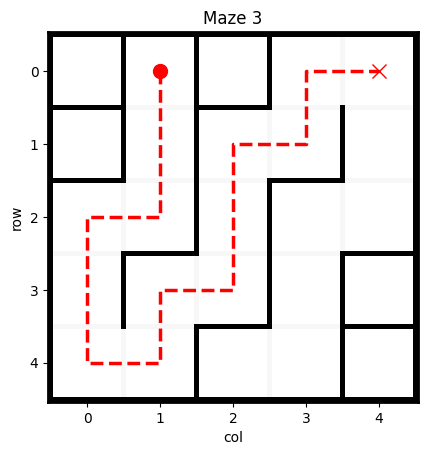
\includegraphics[width=\textwidth]{../mazes/gen_dfs_5x5/figures/maze3.png}
    \caption{Maze 3}
    \label{fig:maze3}
  \end{subfigure}
  \hfill
  \begin{subfigure}[b]{0.45\columnwidth}
    \centering
    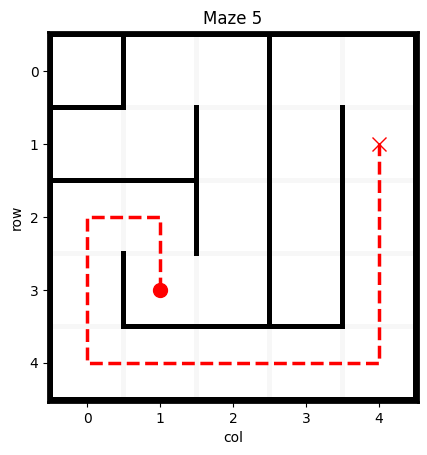
\includegraphics[width=\textwidth]{../mazes/gen_dfs_5x5/figures/maze5.png}
    \caption{Maze 5}
    \label{fig:maze5}
  \end{subfigure}
  \caption{Worst Performing Mazes}
  \label{fig:worst_mazes}
\end{figure}

\begin{figure}[htbp]
  \centering
  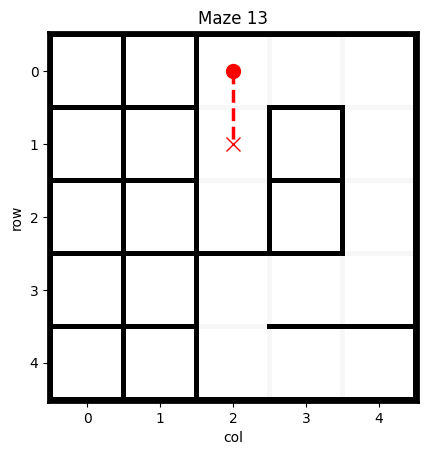
\includegraphics[width=0.45\columnwidth]{../mazes/gen_dfs_5x5/figures/maze13.png}
  \caption{Best Performing Maze}
  \label{fig:best_maze}
\end{figure}

\subsection{Trend Analysis}

The best and worst performing mazes in Figure~\ref{fig:worst_mazes} and Figure~\ref{fig:best_maze} bring up and interesting question whether longer mazes result in lower accuracy. Intuition says yes since there are more places that a Large Language Model can mess up. It could also further complicate any model that thinks more before arriving at an answer. This trend is supported by Figure~\ref{fig:maze_length_accuracy} with an $R^2$ value of 0.827. Not all of the residuals can be accounted for, but it can most likely be attributed to variances between the models and input formats, as well as the variable nature of Large Language Models in general.

This brings up another question on whether a more generally complex maze is less accurate or if path length is the main contributor to reduced accuracy. Figure~\ref{fig:direction_change_accuracy} shows that when accounting for path length, the number of direction changes or turns did not reduce the accuracy of the model responses, except for the notable trivial outliers with extremely short path length, which can most likely be attributed to that rather than them having no direction changes.

\begin{figure}[htbp]
  \centering
  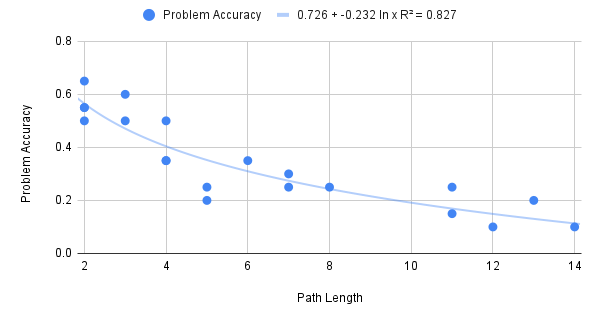
\includegraphics[width=\columnwidth]{Maze Path Length vs. Problem Accuracy.png}
  \caption{Maze Path Length vs. Problem Accuracy. Accuracy trends lower logarithmically or quadratically the longer the path solution is.}
  \label{fig:maze_length_accuracy}
\end{figure}

\begin{figure}[htbp]
  \centering
  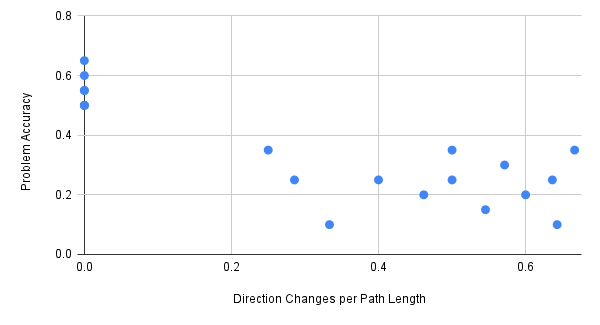
\includegraphics[width=\columnwidth]{Direction Changes per Path Length vs. Problem Accuracy.png}
  \caption{Direction Changes per Path Length vs. Problem Accuracy. No-turn, low-length, trivial problems are higher in accuracy, but there is not an identifiable trend in a higher number of turns reducing accuracy.}
  \label{fig:direction_change_accuracy}
\end{figure}

\section{Conclusion}

Out of the Large Language Models tested, the \texttt{deepseek-v3} model performed best on average, though it was weighed down by its low accuracy on cardinal-based inputs. Cardinal-based inputs have a lower accuracy in general, with coordinate-inputs having a higher accuracy across all models. There's also a high correlation between path length and problem accuracy, with longer maze solutions resulting in worse accuracy. However, no such trend can be identified for the number of turns after accounting for path length.

\subsection{Future Work}

There are many areas this project could be expanded on. Firstly, more models, and potentially more expensive, larger models could be tested on the inputs to see how accuracy is affected. The four models tested were selected due to their similar nature. We are also unsure if cardinal-based inputs were utilized to their full potential. There were many options to alter those inputs, but we were only able to select, test, and one form of them. Additionally, all mazes tested were of the same small 5x5 size. The trend of path length and accuracy could be expanded out to further values. Maze size could also be compared to the accuracy of the different input formats to see if some degrade quicker in accuracy than others.

\section{Acknowledgments}

We thank Michael Igorevich Ivanitskiy for supporting us through Decoding GPT, alongside the other creators of the \texttt{maze-dataset} package~\cite{ivanitskiy}, which made the project possible.

Generative AI was utilized in the creation of this project. GitHub Copilot was used to assist the code portions of this project (though we don't have a saved history), and ChatGPT was also consulted in the formatting of this report.

The work on this project was evenly distributed amongst its authors, split between theoretical and practical focuses accordingly

\begin{thebibliography}{00}

\bibitem{openai}
OpenAI, ``GPT-4 Technical Report,'' \emph{arXiv preprint arXiv:2303.08774}, 2023. [Online]. Available: \url{https://arxiv.org/abs/2303.08774}

\bibitem{srivastava}
A.~Srivastava \emph{et al.}, ``Beyond the Imitation Game: Quantifying and extrapolating the capabilities of language models,'' \emph{arXiv preprint arXiv:2206.04615}, 2022.

\bibitem{liang}
P.~Liang \emph{et al.}, ``Holistic Evaluation of Language Models,'' \emph{arXiv preprint arXiv:2211.09110}, 2022.

\bibitem{tolman} E. C. Tolman, "Cognitive Maps in Rats and Men," Psychol. Rev., vol. 55, no. 4, pp. 189-208, Jul. 1948.

\bibitem{piaget} J. Piaget and B. Inhelder, "The Child's Conception of Space," Int. J. Psychol., vol. 2, no. 3, pp. 241-242, 1967.

\bibitem{stentz} Path-finding Algorithms: A. Stentz, "Optimal and Efficient Path Planning for Partially Known Environments," in IEEE International Conference on Robotics and Automation, 1994, pp. 3310-3317.

\bibitem{hendrycks}
D.~Hendrycks \emph{et al.}, ``Measuring Massive Multitask Language Understanding,'' \emph{arXiv preprint arXiv:2009.03300}, 2021.

\bibitem{ahn}
M.~Ahn \emph{et al.}, ``Do As I Can, Not As I Say: Grounding Language in Robotic Affordances,'' \emph{arXiv preprint arXiv:2204.01691}, 2022.

\bibitem{yao}
S.~Yao \emph{et al.}, ``ReAct: Synergizing Reasoning and Acting in Language Models,'' \emph{arXiv preprint arXiv:2210.03629}, 2022.

\bibitem{ivanitskiy}
M.~I. Ivanitskiy \emph{et al.}, ``A configurable library for generating and manipulating maze datasets,'' \emph{arXiv preprint arXiv:2309.10498}, 2023. [Online]. Available: \url{https://arxiv.org/abs/2309.10498}

\bibitem{deepseek} DeepSeek-V3, DeepSeek, 2024. [Online]. Available: \url{https://github.com/deepseek-ai/DeepSeek-V3}

\bibitem{gemini} Gemini 2.0, Google DeepMind, 2024. [Online]. Available: \url{https://deepmind.google/technologies/gemini/}

\bibitem{gpt4omini} GPT-4o Mini, OpenAI, 2024. [Online]. Available: \url{https://openai.com/blog/gpt-4o}

\bibitem{llama4scout} LLaMA 4 Scout 17B, DeepInfra, 2024. [Online]. Available: \url{https://deepinfra.com/models/meta-llama/llama-4-scout-17b}

\bibitem{openaiapi} OpenAI Python API, OpenAI, 2024. [Online]. Available: \url{https://pypi.org/project/openai/}

\bibitem{promptmetheus} Promptmetheus LLM Index, “LLM Index – Parameter Counts, Licensing, and Context Lengths,” 2024. [Online]. Available: \url{https://promptmetheus.com/resources/llm-index}


\end{thebibliography}

\end{document}
